% XeLaTeX

\documentclass{article}
\usepackage{ctex}
\usepackage{xypic}
\usepackage{amsfonts,amssymb}
\usepackage{multirow}
\usepackage{geometry}
\usepackage{graphicx}
\usepackage{listings}
\usepackage{lipsum}
\usepackage{courier}
\usepackage{fancyvrb}
\usepackage{etoolbox}


\linespread{1.2}
\geometry{left=3cm,right=2.5cm,top=2.5cm,bottom=2.5cm}

\makeatletter
\patchcmd{\FV@SetupFont}
  {\FV@BaseLineStretch}
  {\fontencoding{T1}\FV@BaseLineStretch}
  {}{}
\makeatother

\lstset{basicstyle=\small\fontencoding{T1}\ttfamily,breaklines=true}
\lstset{numbers=left,frame=shadowbox,tabsize=4}
%\lstset{extendedchars=false}
\begin{document}

\title{实验九 \text{ } 计数器的设计 \text{ } 实验报告}
\author {16337233 王凯祺}
\maketitle

\section{实验目的}

熟悉 JK 触发器的逻辑功能,掌握 JK 触发器构成异步计数器和同步计数器。

\section{实验仪器}

1. 实验箱、万用表、示波器

2. 74LS73、74LS00、74LS08、74LS20

\section{实验内容}

\subsection{用 JK 触发器设计一个 16 进制异步计数器}

将前一个 JK 触发器的输出接到后一个 JK 触发器的 J 端和 K 端,则当前一个 JK 触发器输出的下降沿到达时,后一个 JK 触发器的输出反转。

\subsubsection{Proteus 实验设计}

\begin{figure}[!hbp]
  \centering
  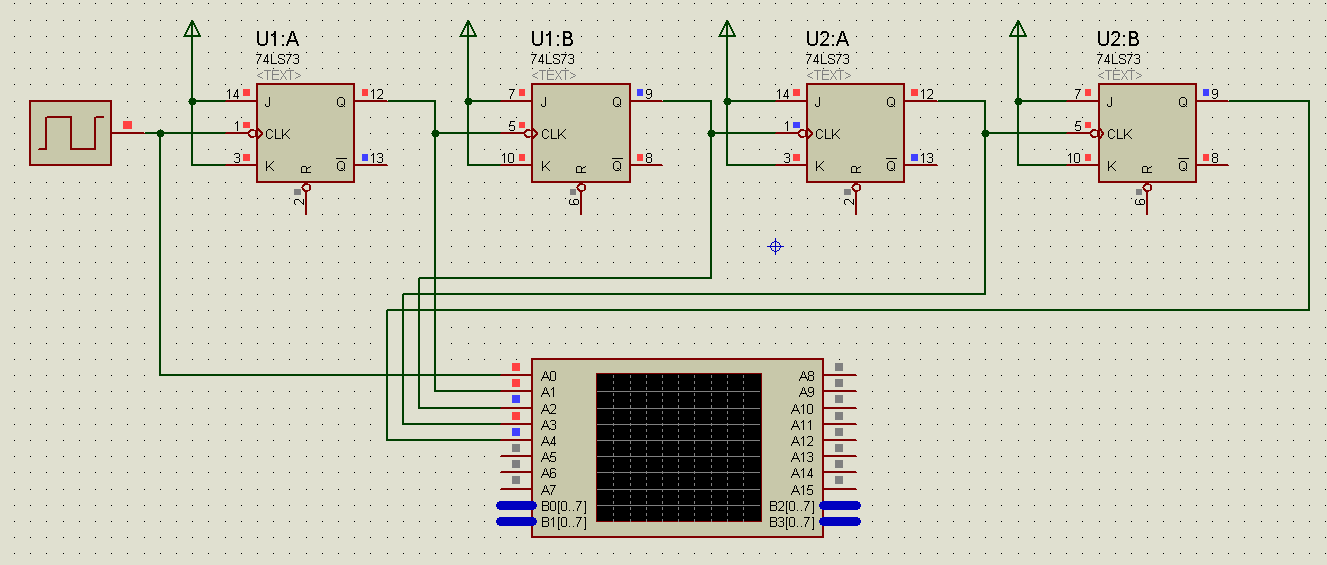
\includegraphics[scale=0.3]{1/1.png}
\end{figure}

\newpage

\subsubsection{Proteus 逻辑分析仪}

\begin{figure}[!hbp]
  \centering
  
\includegraphics[scale=0.5]{1/2.png}
\end{figure}

\subsubsection{实验板实现——逻辑分析仪}

\begin{figure}[!hbp]
  \centering
  \includegraphics[scale=0.5]{1/DS2_QuickPrint1.png}
\end{figure}

\newpage

\subsection{用 JK 触发器设计一个 16 进制同步计数器}

\subsubsection{次态表}

\begin{table}[!hbp]
\centering
\begin{tabular}{|c|c|c|c||c|c|c|c|}
\hline
$Q_3$ & $Q_2$ & $Q_1$ & $Q_0$ & $Q_3^+$ & $Q_2^+$ & $Q_1^+$ & $Q_0^+$ \\
\hline
\hline
0 & 0 & 0 & 0 & 0 & 0 & 0 & 1 \\
\hline
0 & 0 & 0 & 1 & 0 & 0 & 1 & 0 \\
\hline
0 & 0 & 1 & 0 & 0 & 0 & 1 & 1 \\
\hline
0 & 0 & 1 & 1 & 0 & 1 & 0 & 0 \\
\hline
0 & 1 & 0 & 0 & 0 & 1 & 0 & 1 \\
\hline
0 & 1 & 0 & 1 & 0 & 1 & 1 & 0 \\
\hline
0 & 1 & 1 & 0 & 0 & 1 & 1 & 1 \\
\hline
0 & 1 & 1 & 1 & 1 & 0 & 0 & 0 \\
\hline
1 & 0 & 0 & 0 & 1 & 0 & 0 & 1 \\
\hline
1 & 0 & 0 & 1 & 1 & 0 & 1 & 0 \\
\hline
1 & 0 & 1 & 0 & 1 & 0 & 1 & 1 \\
\hline
1 & 0 & 1 & 1 & 1 & 1 & 0 & 0 \\
\hline
1 & 1 & 0 & 0 & 1 & 1 & 0 & 1 \\
\hline
1 & 1 & 0 & 1 & 1 & 1 & 1 & 0 \\
\hline
1 & 1 & 1 & 0 & 1 & 1 & 1 & 1 \\
\hline
1 & 1 & 1 & 1 & 0 & 0 & 0 & 0 \\
\hline
\end{tabular}
\end{table}

\subsubsection{触发器转换表}

\begin{table}[!hbp]
\centering
\begin{tabular}{|c|c||c|c|}
\hline
$Q$ & $Q^+$ & J & K \\
\hline
\hline
0 & 0 & 0 & X \\
\hline
0 & 1 & 1 & X \\
\hline
1 & 0 & X & 1 \\
\hline
1 & 1 & X & 0 \\
\hline
\end{tabular}
\end{table}

\newpage

\subsubsection{卡诺图化简}

\begin{figure}[!hbp]
  \centering
  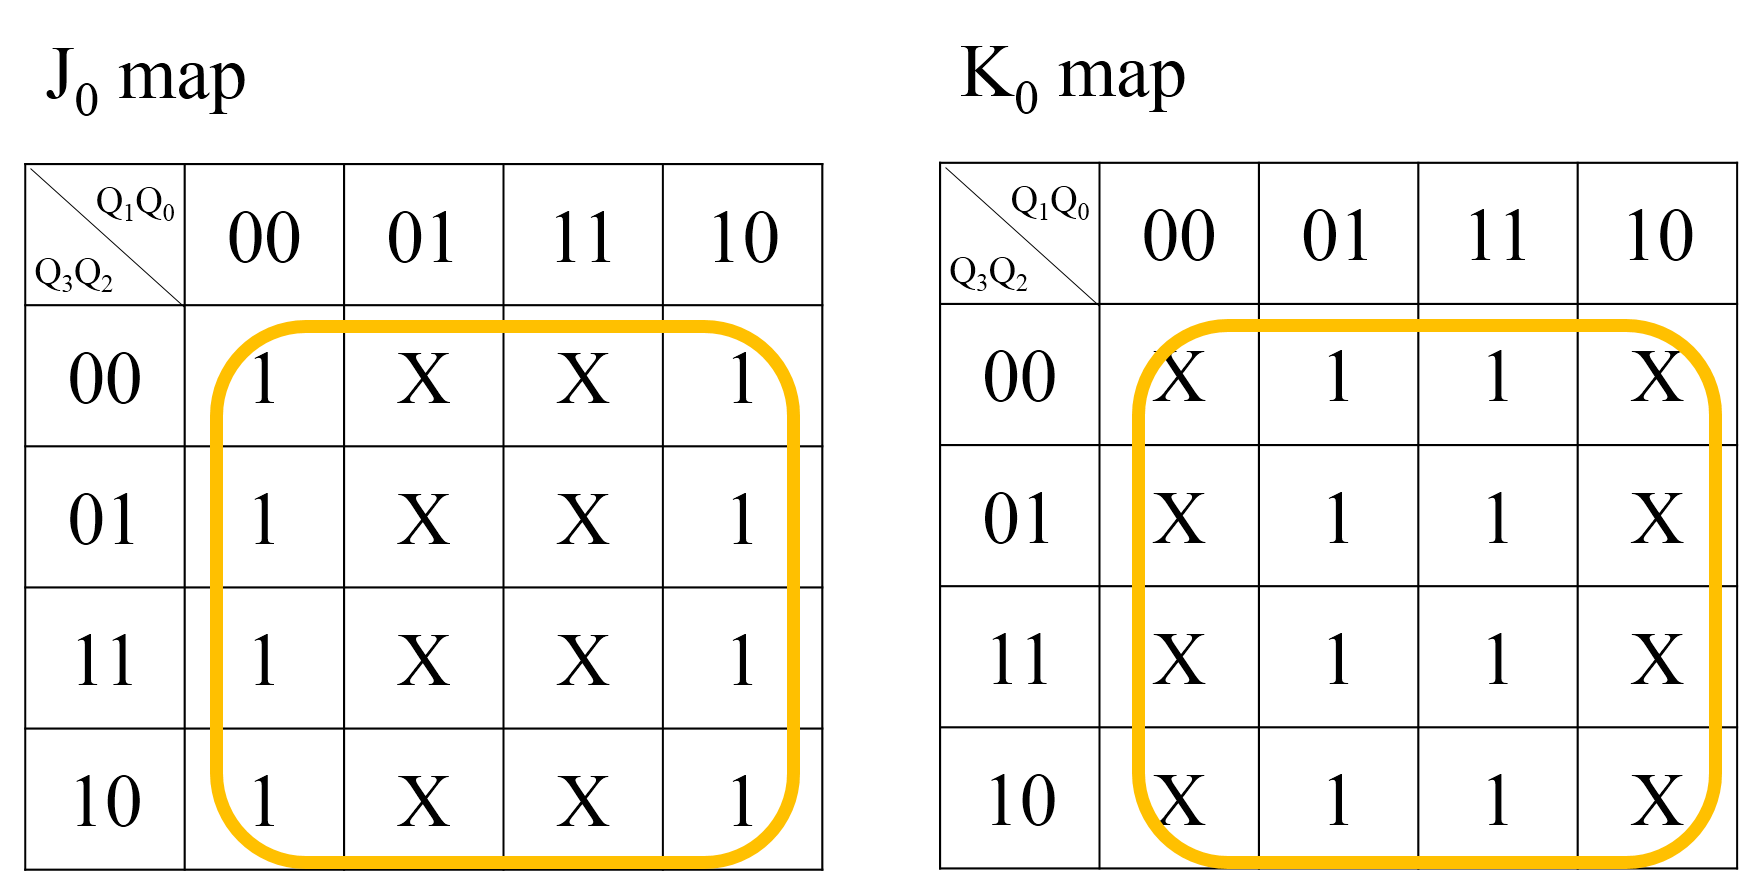
\includegraphics[scale=0.5]{2/k1.png}
\end{figure}

\begin{figure}[!hbp]
  \centering
  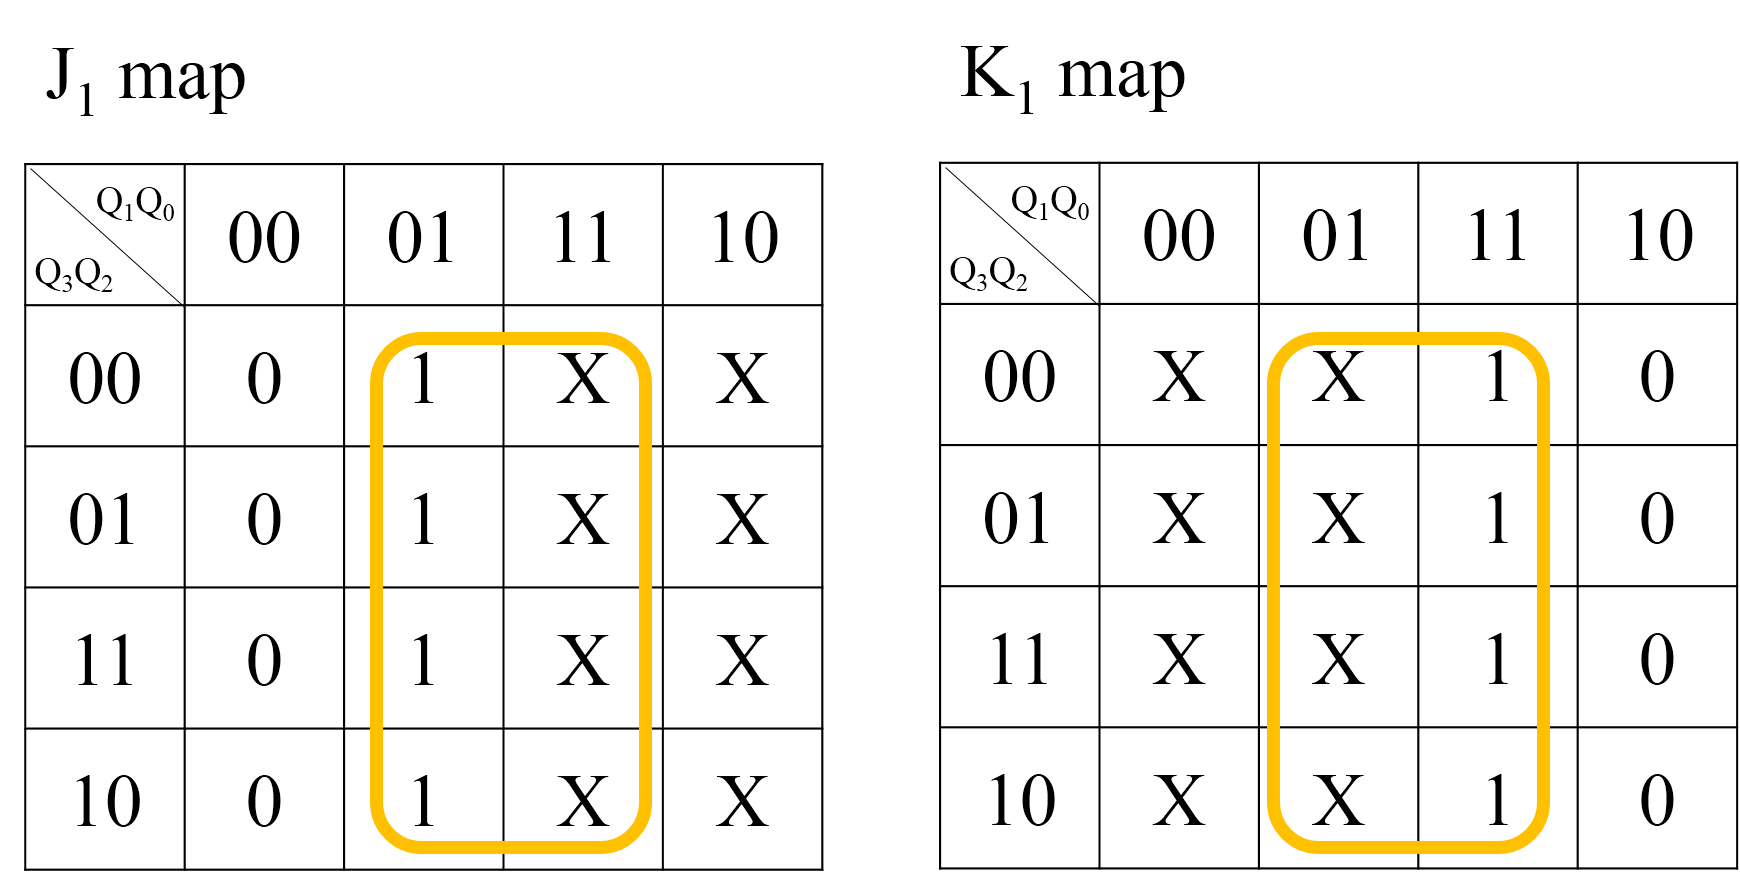
\includegraphics[scale=0.5]{2/k2.png}
\end{figure}

\newpage

\begin{figure}[!hbp]
  \centering
  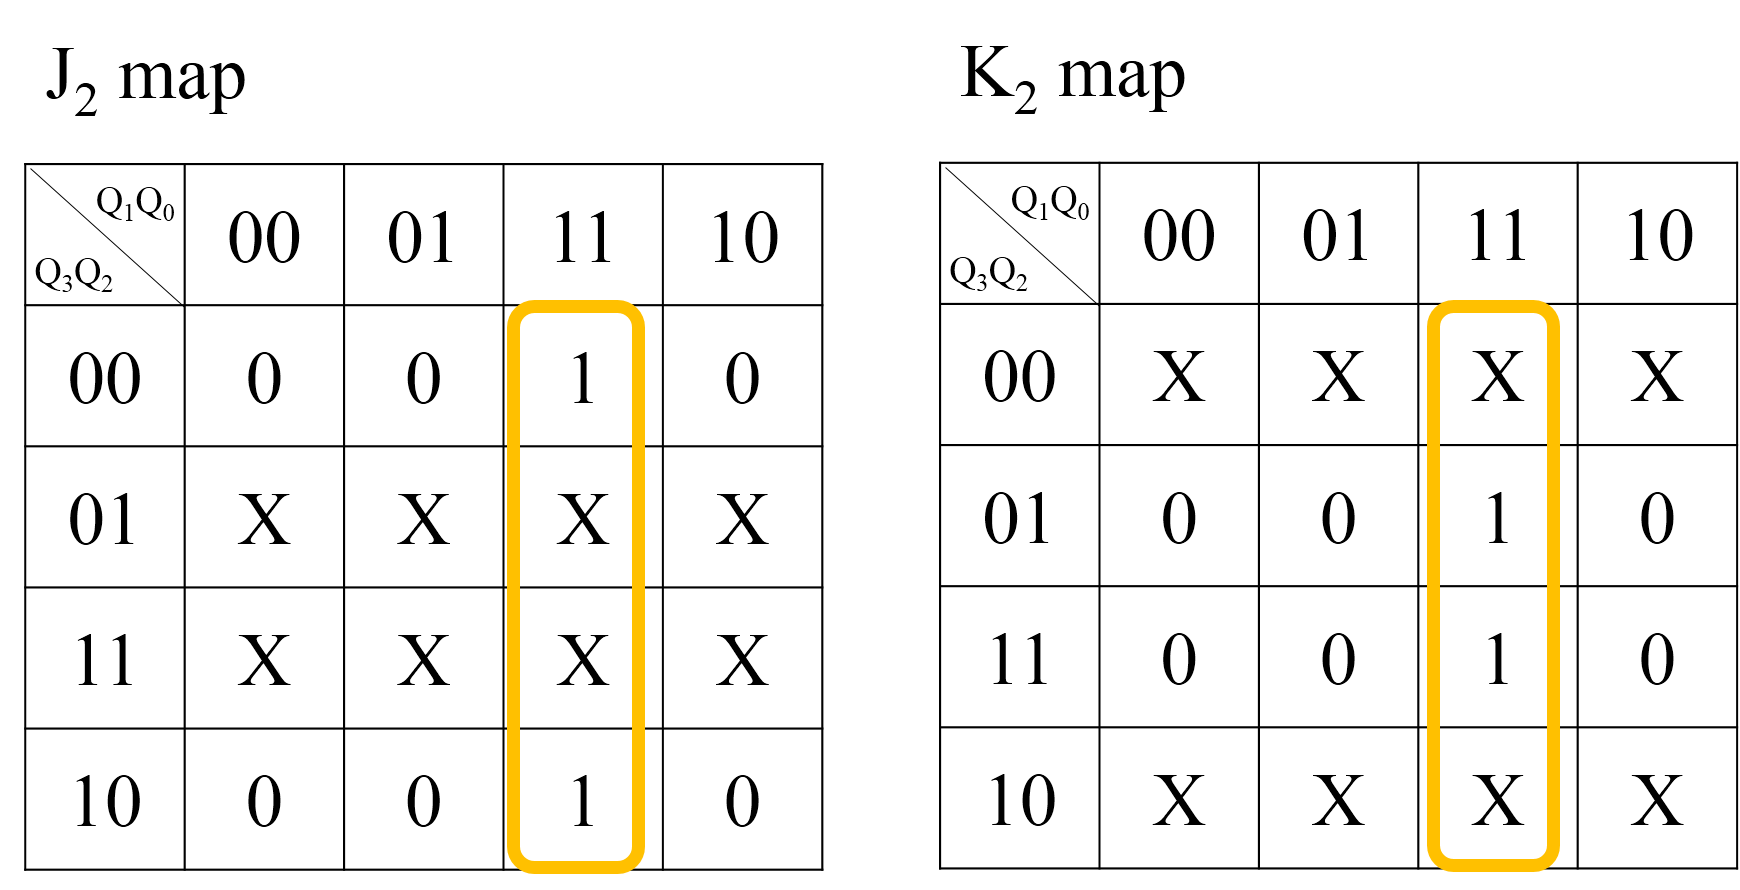
\includegraphics[scale=0.5]{2/k3.png}
\end{figure}

\begin{figure}[!hbp]
  \centering
  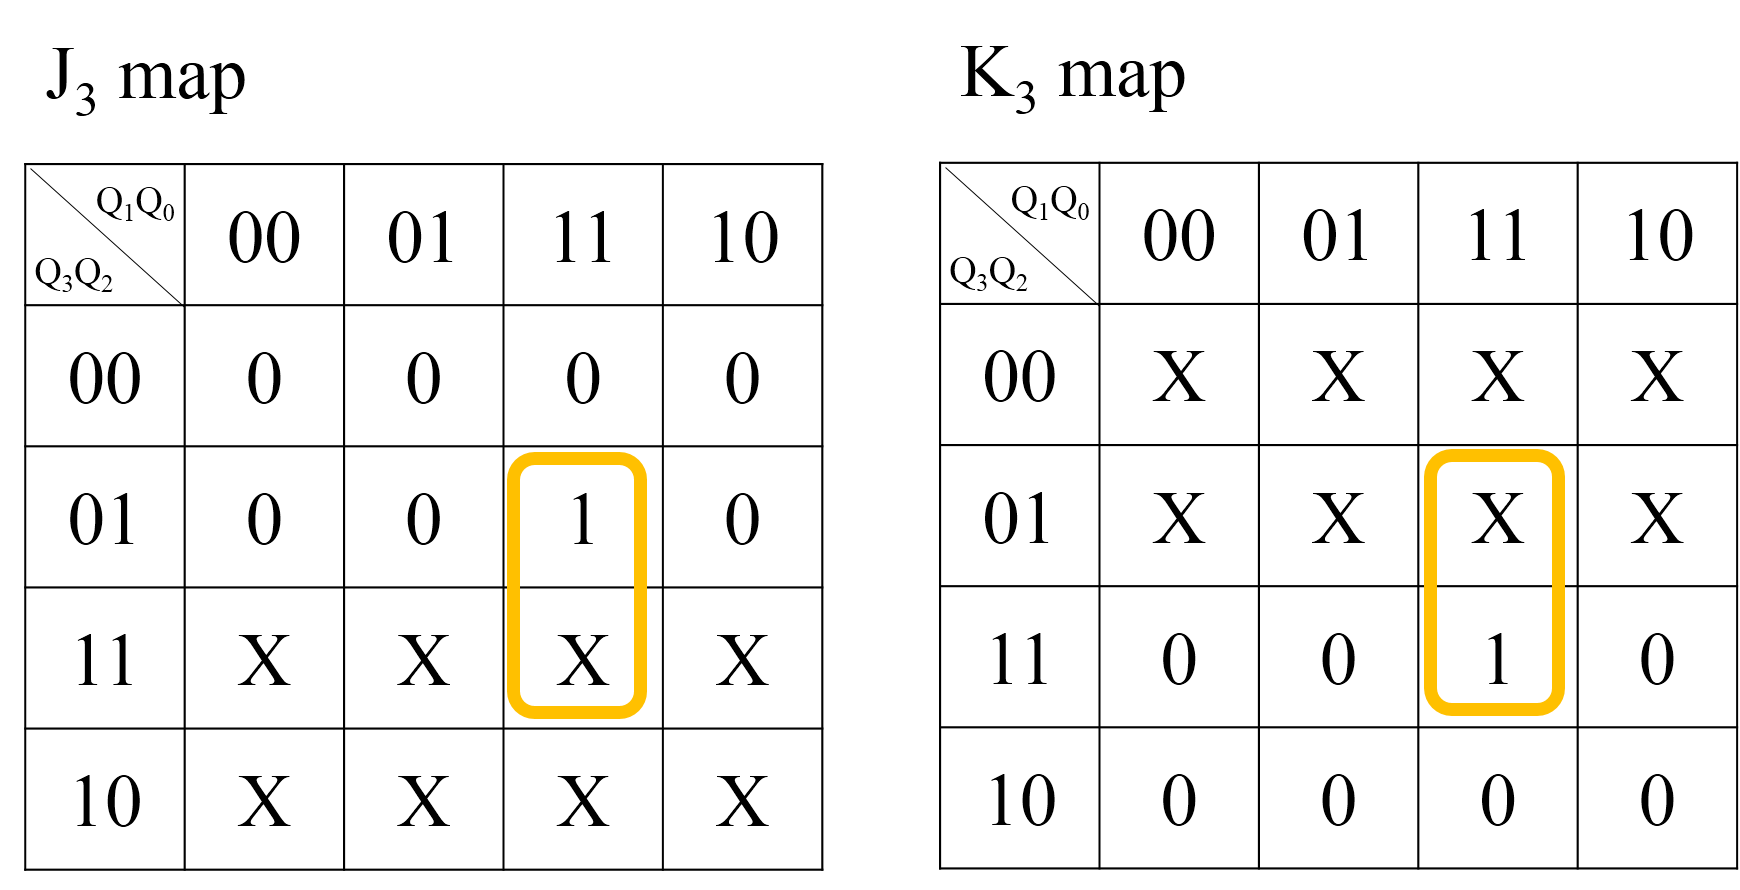
\includegraphics[scale=0.5]{2/k4.png}
\end{figure}

\subsubsection{驱动方程}

$J_0 = 1$

$K_0 = 1$

$J_1 = Q_0$

$K_1 = Q_0$

$J_2 = Q_1 \cdot Q_0$

$K_2 = Q_1 \cdot Q_0$

$J_3 = Q_2 \cdot Q_1 \cdot Q_0$

$K_3 = Q_2 \cdot Q_1 \cdot Q_0$

\newpage

\subsubsection{电路图}

\begin{figure}[!hbp]
  \centering
  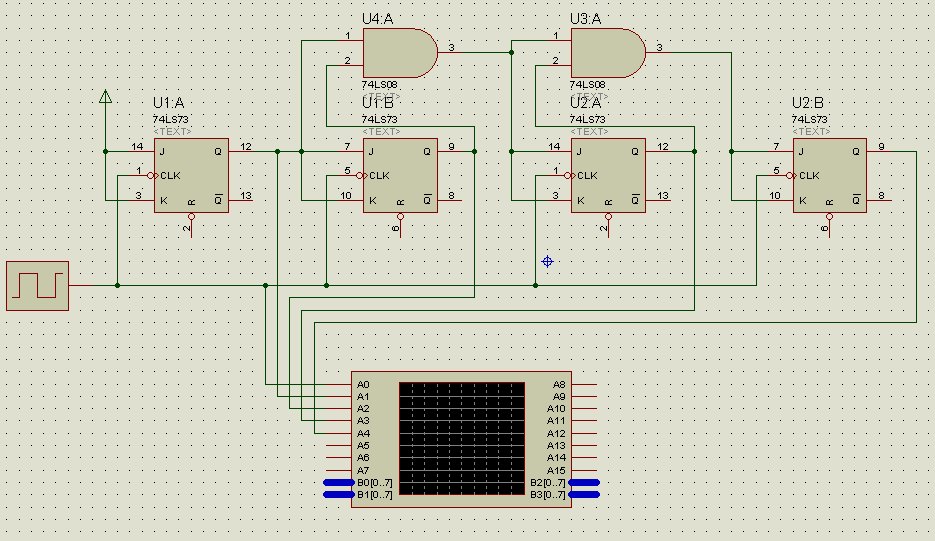
\includegraphics[scale=0.4]{2/1.png}
\end{figure}

\subsubsection{Proteus 逻辑分析仪}

\begin{figure}[!hbp]
  \centering
  
\includegraphics[scale=0.5]{2/2.png}
\end{figure}

\newpage

\subsubsection{实验板实现——逻辑分析仪}

\begin{figure}[!hbp]
  \centering
  \includegraphics[scale=0.5]{2/DS2_QuickPrint2.png}
\end{figure}

\newpage

\subsection{用 JK 触发器设计一个具有右移功能的计数器}


\subsubsection{次态表}

\begin{table}[!hbp]
\centering
\begin{tabular}{|c|c|c|c||c|c|c|c|}
\hline
$Q_3$ & $Q_2$ & $Q_1$ & $Q_0$ & $Q_3^+$ & $Q_2^+$ & $Q_1^+$ & $Q_0^+$ \\
\hline
\hline
0 & 0 & 0 & 0 & $D_{SR}$ & 0 & 0 & 0 \\
\hline
0 & 0 & 0 & 1 & $D_{SR}$ & 0 & 0 & 0 \\
\hline
0 & 0 & 1 & 0 & $D_{SR}$ & 0 & 0 & 1 \\
\hline
0 & 0 & 1 & 1 & $D_{SR}$ & 0 & 0 & 1 \\
\hline
0 & 1 & 0 & 0 & $D_{SR}$ & 0 & 1 & 0 \\
\hline
0 & 1 & 0 & 1 & $D_{SR}$ & 0 & 1 & 0 \\
\hline
0 & 1 & 1 & 0 & $D_{SR}$ & 0 & 1 & 1 \\
\hline
0 & 1 & 1 & 1 & $D_{SR}$ & 0 & 1 & 1 \\
\hline
1 & 0 & 0 & 0 & $D_{SR}$ & 1 & 0 & 0 \\
\hline
1 & 0 & 0 & 1 & $D_{SR}$ & 1 & 0 & 0 \\
\hline
1 & 0 & 1 & 0 & $D_{SR}$ & 1 & 0 & 1 \\
\hline
1 & 0 & 1 & 1 & $D_{SR}$ & 1 & 0 & 1 \\
\hline
1 & 1 & 0 & 0 & $D_{SR}$ & 1 & 1 & 0 \\
\hline
1 & 1 & 0 & 1 & $D_{SR}$ & 1 & 1 & 0 \\
\hline
1 & 1 & 1 & 0 & $D_{SR}$ & 1 & 1 & 1 \\
\hline
1 & 1 & 1 & 1 & $D_{SR}$ & 1 & 1 & 1 \\
\hline
\end{tabular}
\end{table}

\subsubsection{触发器转换表}

\begin{table}[!hbp]
\centering
\begin{tabular}{|c|c||c|c|}
\hline
$Q$ & $Q^+$ & J & K \\
\hline
\hline
0 & 0 & 0 & X \\
\hline
0 & 1 & 1 & X \\
\hline
1 & 0 & X & 1 \\
\hline
1 & 1 & X & 0 \\
\hline
\end{tabular}
\end{table}

\newpage

\subsubsection{卡诺图化简}

\begin{figure}[!hbp]
  \centering
  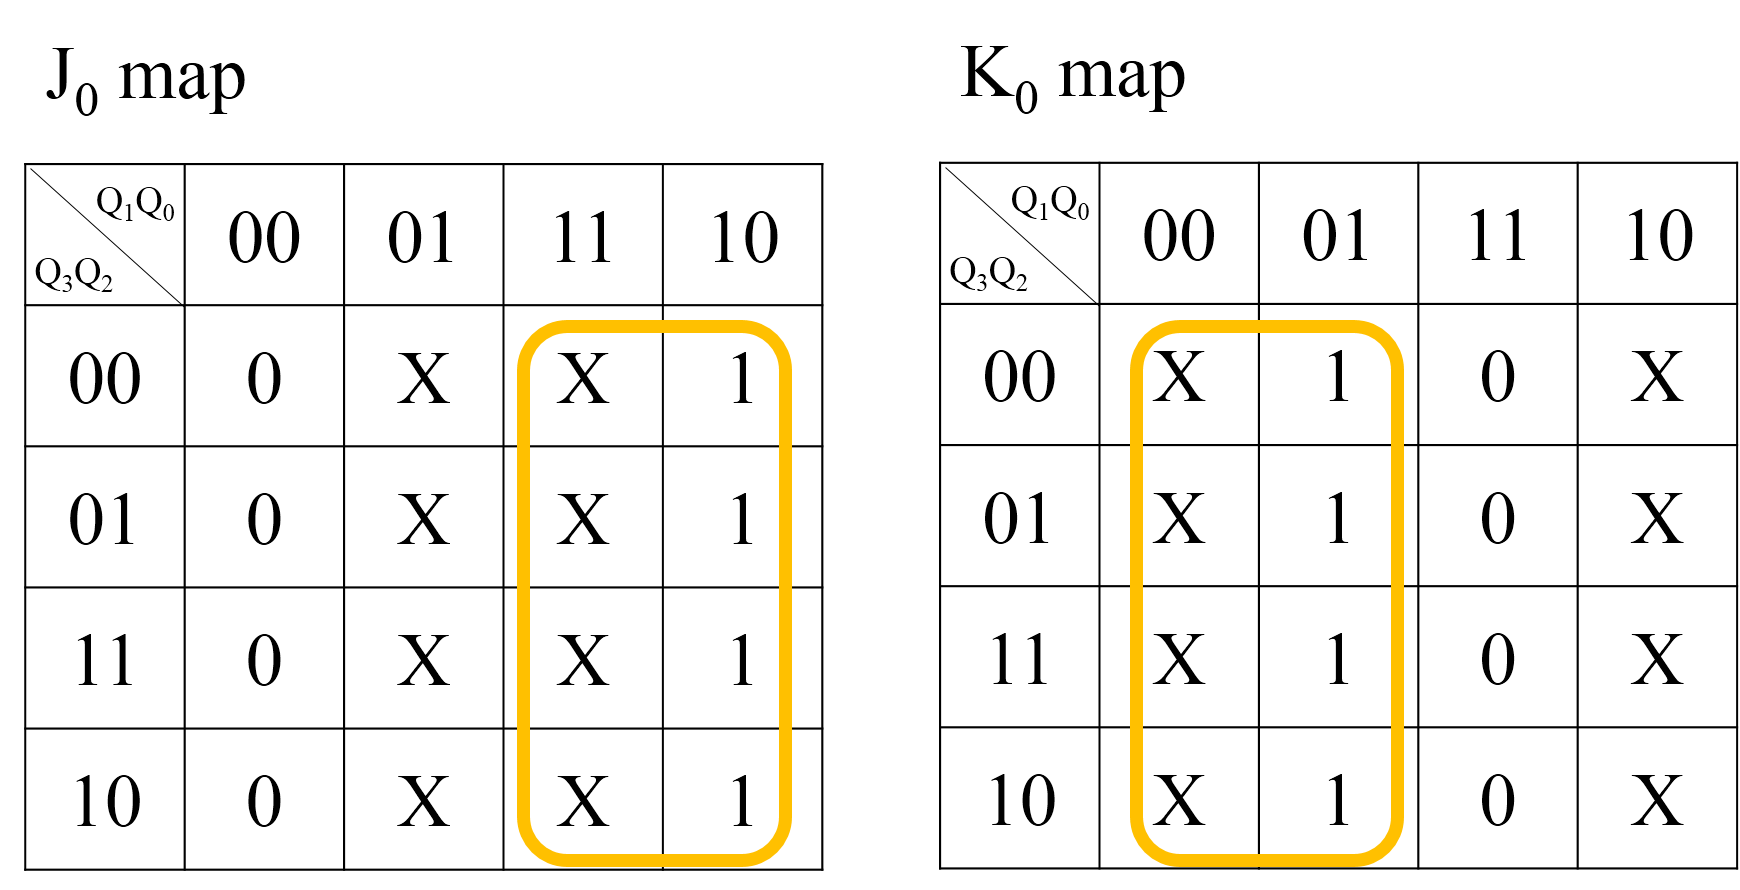
\includegraphics[scale=0.5]{3/k1.png}
\end{figure}

\begin{figure}[!hbp]
  \centering
  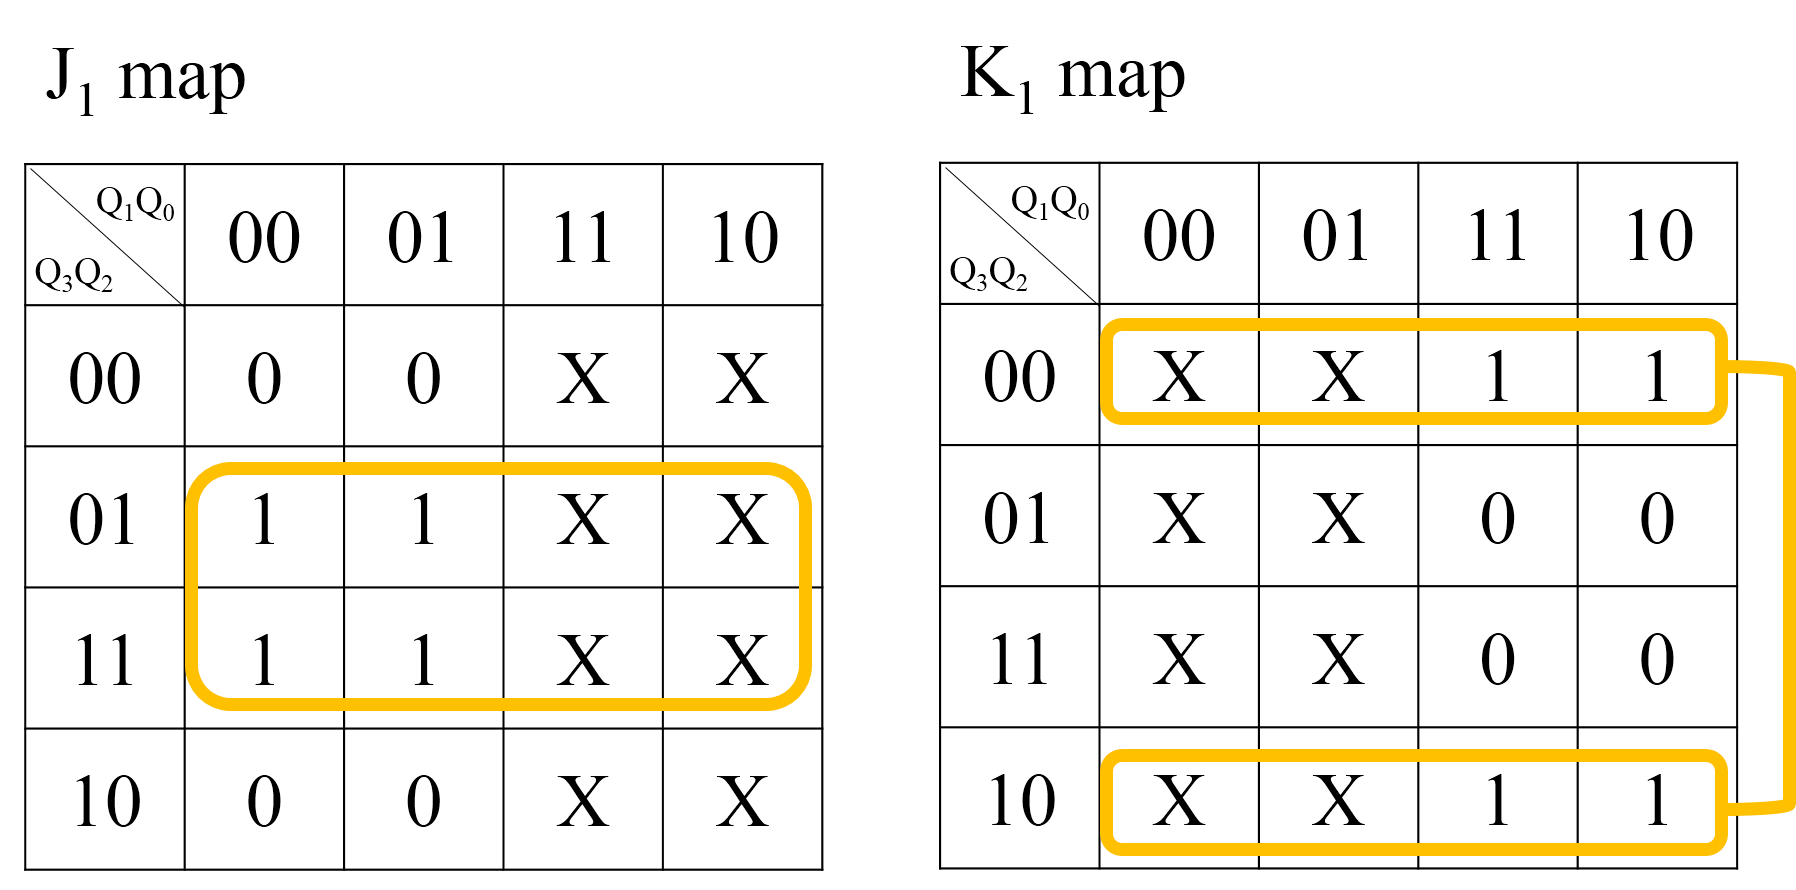
\includegraphics[scale=0.5]{3/k2.png}
\end{figure}

\newpage

\begin{figure}[!hbp]
  \centering
  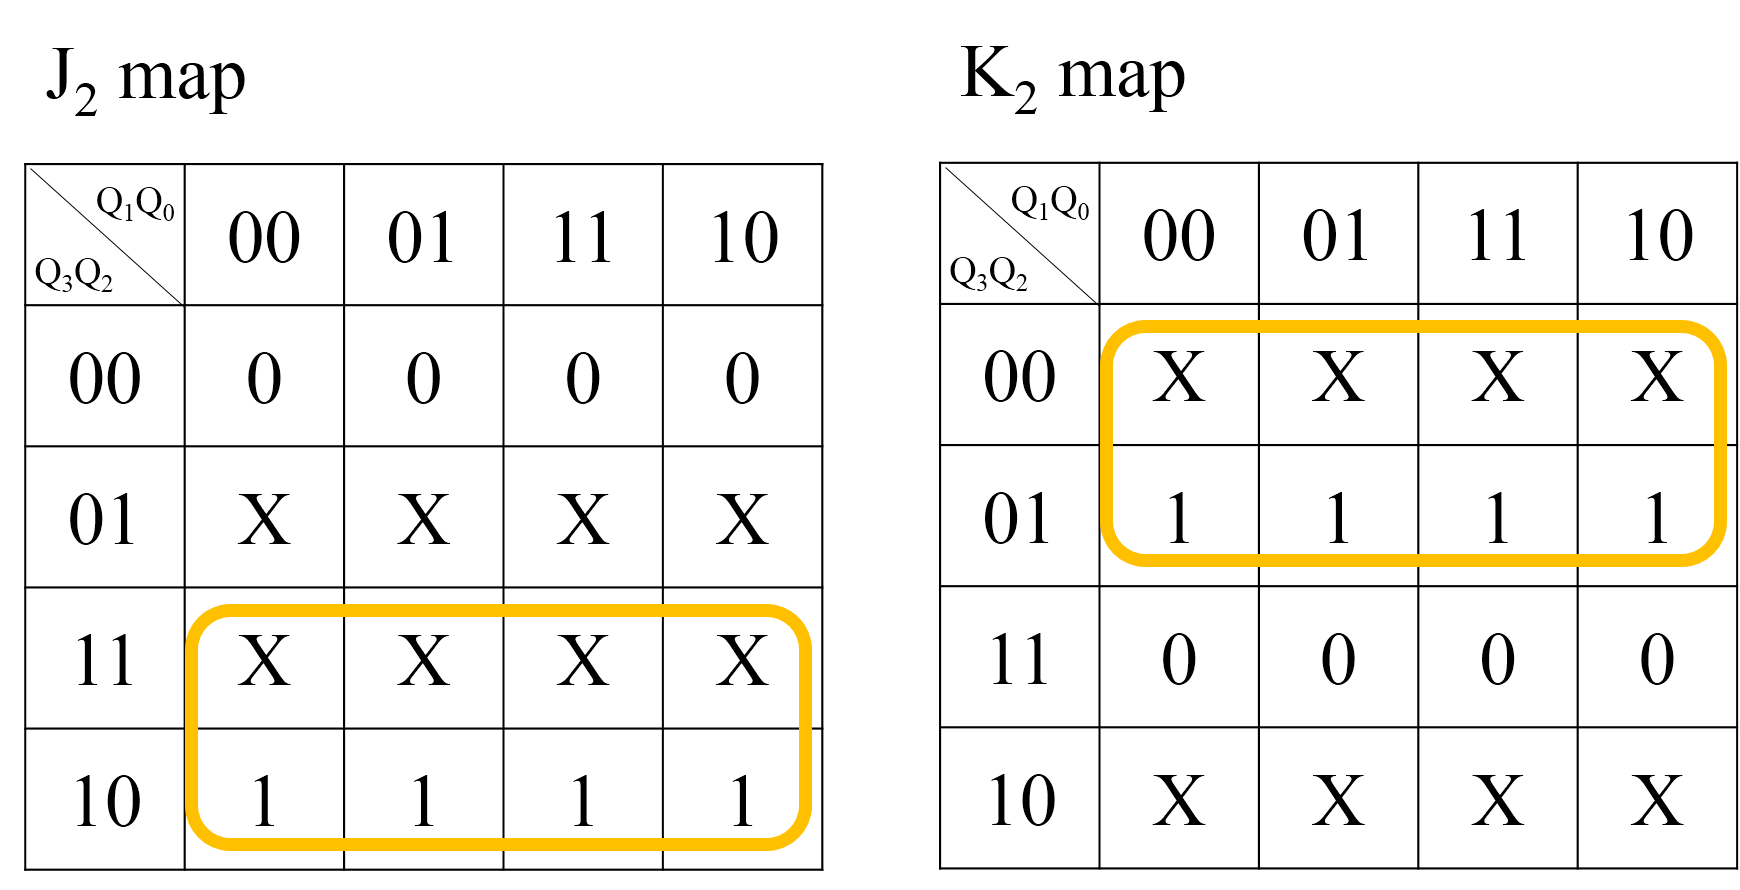
\includegraphics[scale=0.5]{3/k3.png}
\end{figure}

\begin{figure}[!hbp]
  \centering
  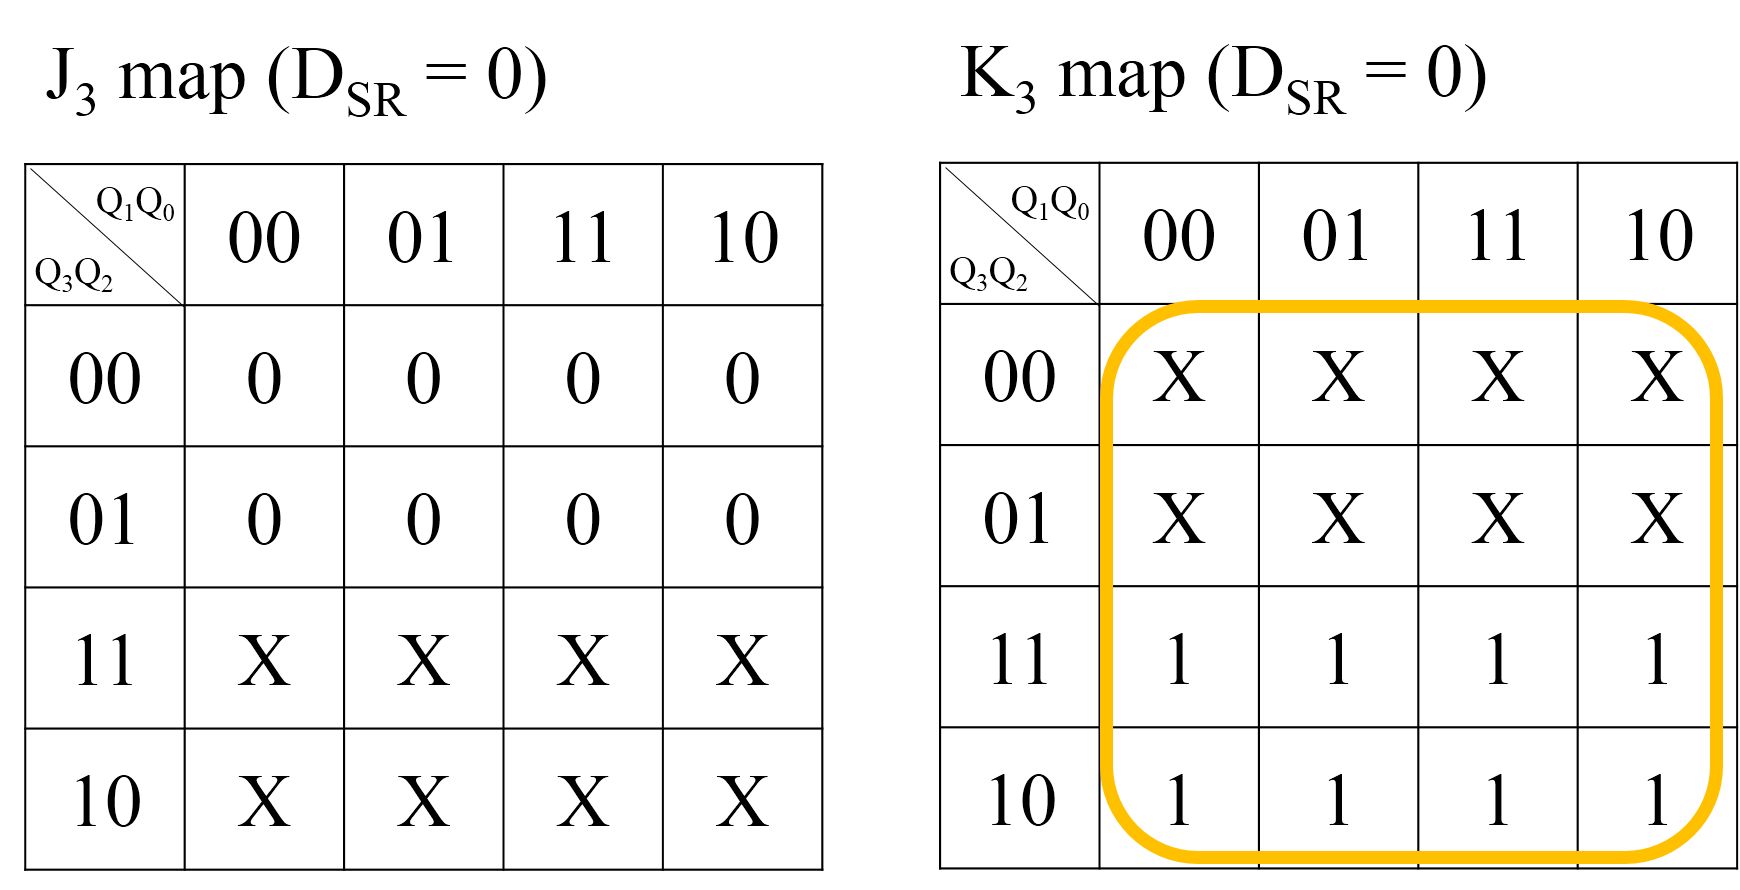
\includegraphics[scale=0.5]{3/k4.png}
\end{figure}

\newpage

\begin{figure}[!hbp]
  \centering
  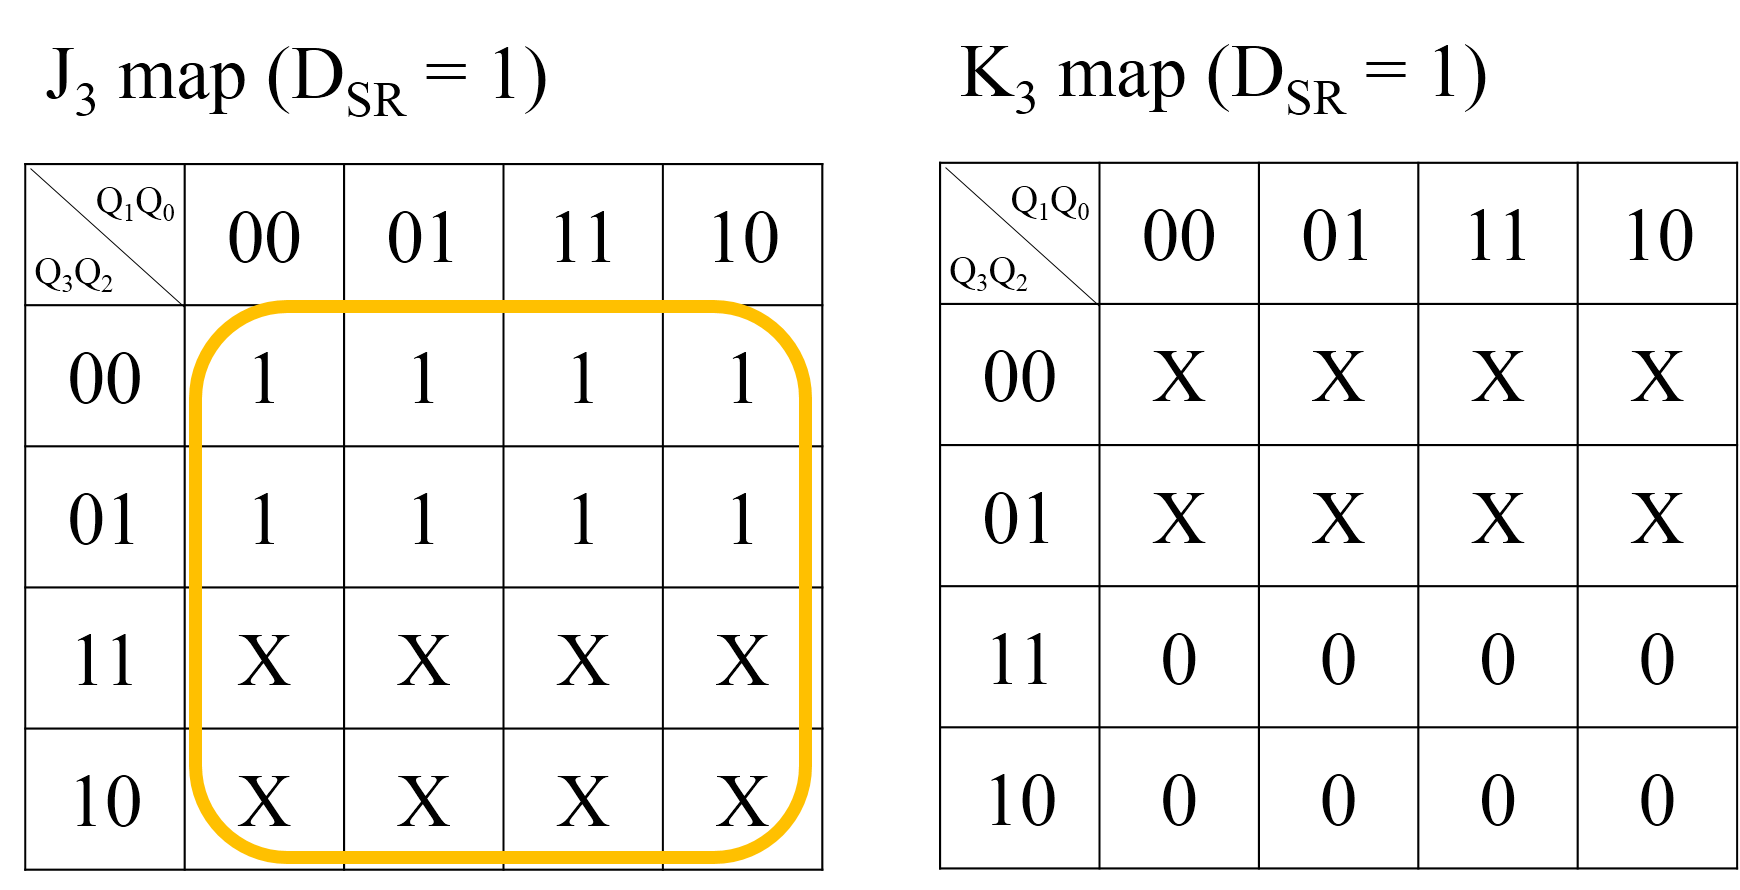
\includegraphics[scale=0.5]{3/k5.png}
\end{figure}

\subsubsection{驱动方程}

$J_0 = Q_1$

$K_0 = \overline{Q_1}$

$J_1 = Q_2$

$K_1 = \overline{Q_2}$

$J_2 = Q_3$

$K_2 = \overline{Q_3}$

$J_3 = D_{SR}$

$K_3 = \overline{D_{SR}}$

\subsubsection{电路图}

\begin{figure}[!hbp]
  \centering
  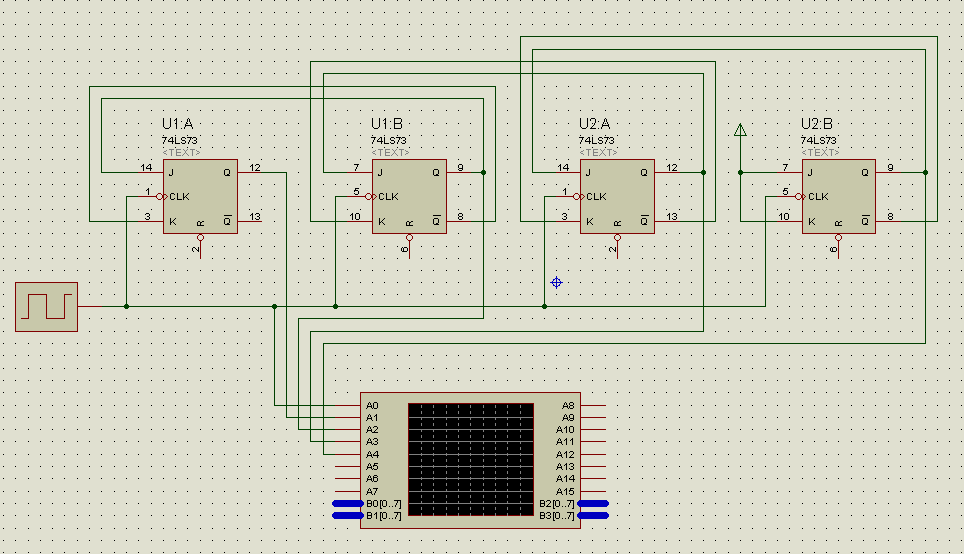
\includegraphics[scale=0.35]{3/1.png}
\end{figure}

\newpage

\subsection{用 JK 触发器设计一个特殊的 12 进制同步计数器}

\subsubsection{状态转换图}

01 $\rightarrow$ 02 $\rightarrow$ 03 $\rightarrow$ 04 $\rightarrow$ 05 $\rightarrow$ 06 $\rightarrow$ 07 $\rightarrow$ 08 $\rightarrow$ 09 $\rightarrow$ 10 $\rightarrow$ 11 $\rightarrow$ 12 $\rightarrow$ 01 $\rightarrow \cdots$

\subsubsection{次态表}

\begin{table}[!hbp]
\centering
\begin{tabular}{|c|c|c|c||c|c|c|c|}
\hline
$Q_3$ & $Q_2$ & $Q_1$ & $Q_0$ & $Q_3^+$ & $Q_2^+$ & $Q_1^+$ & $Q_0^+$ \\
\hline
\hline
0 & 0 & 0 & 0 & 0 & 0 & 0 & 1 \\
\hline
0 & 0 & 0 & 1 & 0 & 0 & 1 & 0 \\
\hline
0 & 0 & 1 & 0 & 0 & 0 & 1 & 1 \\
\hline
0 & 0 & 1 & 1 & 0 & 1 & 0 & 0 \\
\hline
0 & 1 & 0 & 0 & 0 & 1 & 0 & 1 \\
\hline
0 & 1 & 0 & 1 & 0 & 1 & 1 & 0 \\
\hline
0 & 1 & 1 & 0 & 0 & 1 & 1 & 1 \\
\hline
0 & 1 & 1 & 1 & 1 & 0 & 0 & 0 \\
\hline
1 & 0 & 0 & 0 & 1 & 0 & 0 & 1 \\
\hline
1 & 0 & 0 & 1 & 1 & 0 & 1 & 0 \\
\hline
1 & 0 & 1 & 0 & 1 & 0 & 1 & 1 \\
\hline
1 & 0 & 1 & 1 & 1 & 1 & 0 & 0 \\
\hline
1 & 1 & 0 & 0 & 0 & 0 & 0 & 1 \\
\hline
\end{tabular}
\end{table}

\subsubsection{触发器转换表}

\begin{table}[!hbp]
\centering
\begin{tabular}{|c|c||c|c|}
\hline
$Q$ & $Q^+$ & J & K \\
\hline
\hline
0 & 0 & 0 & X \\
\hline
0 & 1 & 1 & X \\
\hline
1 & 0 & X & 1 \\
\hline
1 & 1 & X & 0 \\
\hline
\end{tabular}
\end{table}

\newpage

\subsubsection{卡诺图化简}

\begin{figure}[!hbp]
  \centering
  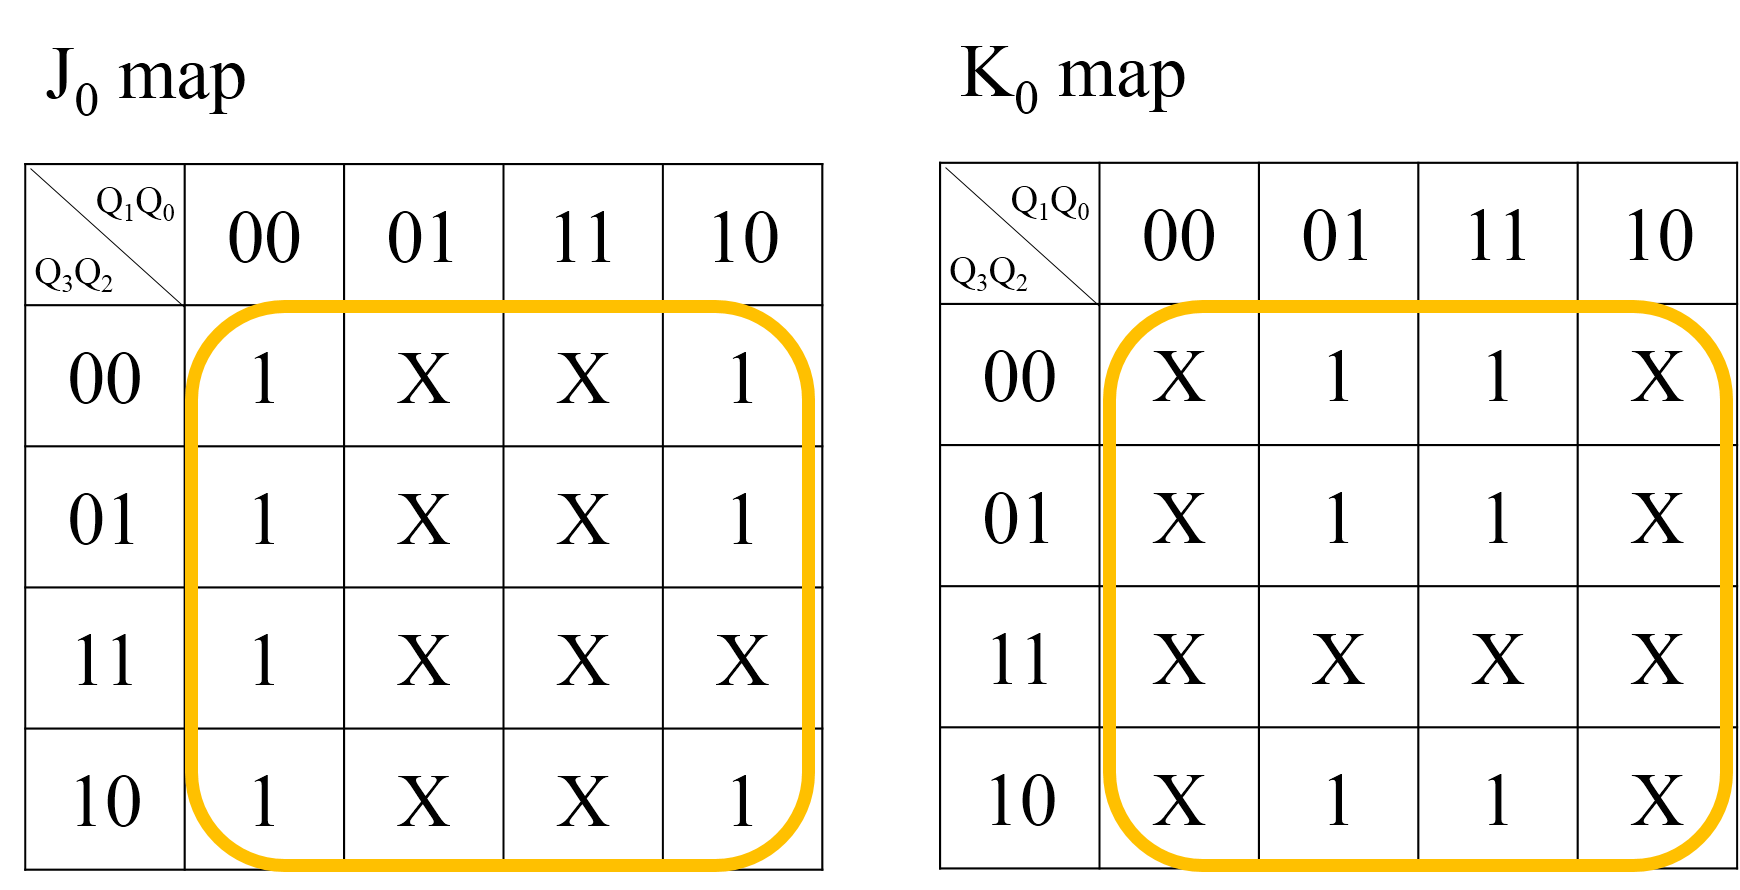
\includegraphics[scale=0.5]{4/k1.png}
\end{figure}

\begin{figure}[!hbp]
  \centering
  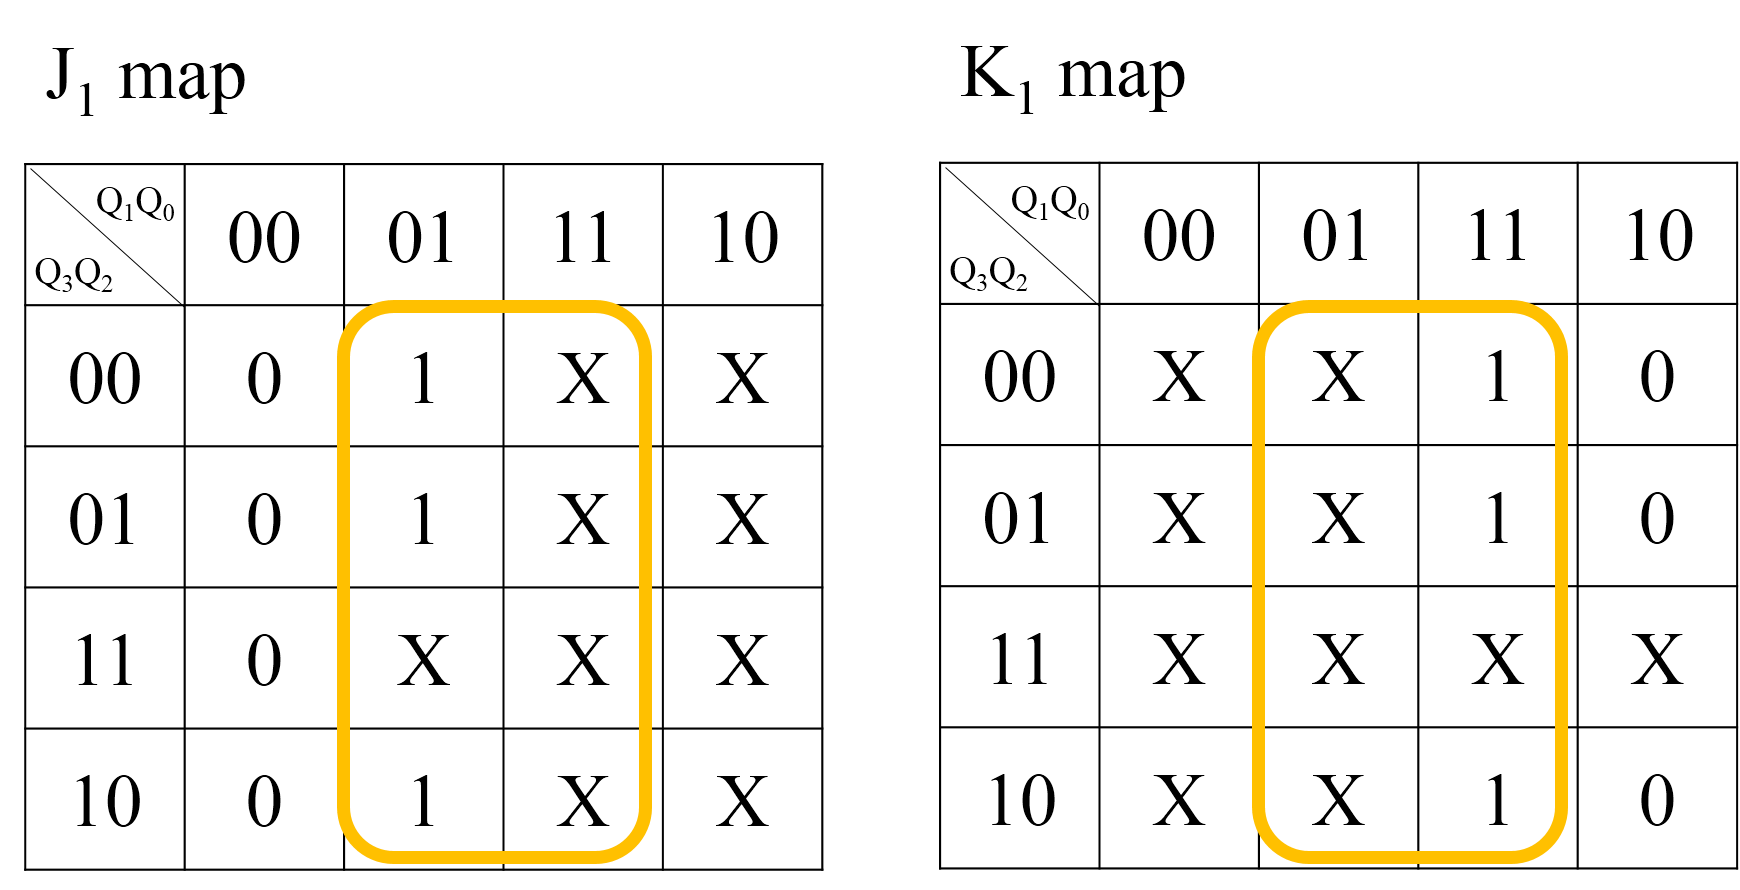
\includegraphics[scale=0.5]{4/k2.png}
\end{figure}

\newpage

\begin{figure}[!hbp]
  \centering
  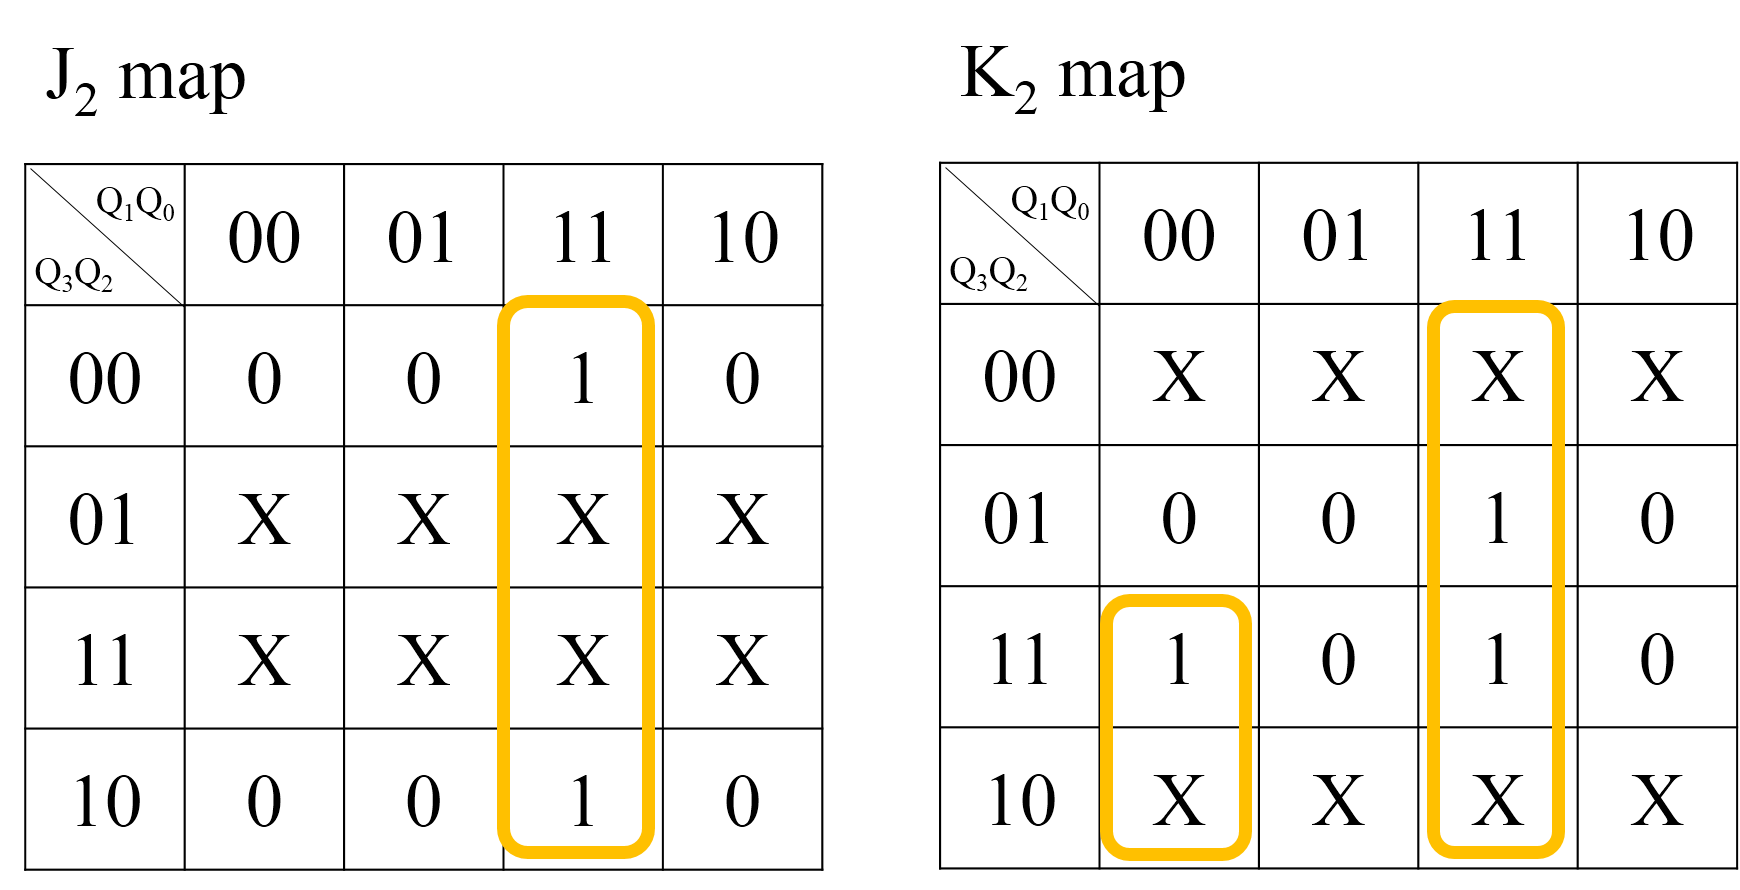
\includegraphics[scale=0.5]{4/k3.png}
\end{figure}

\begin{figure}[!hbp]
  \centering
  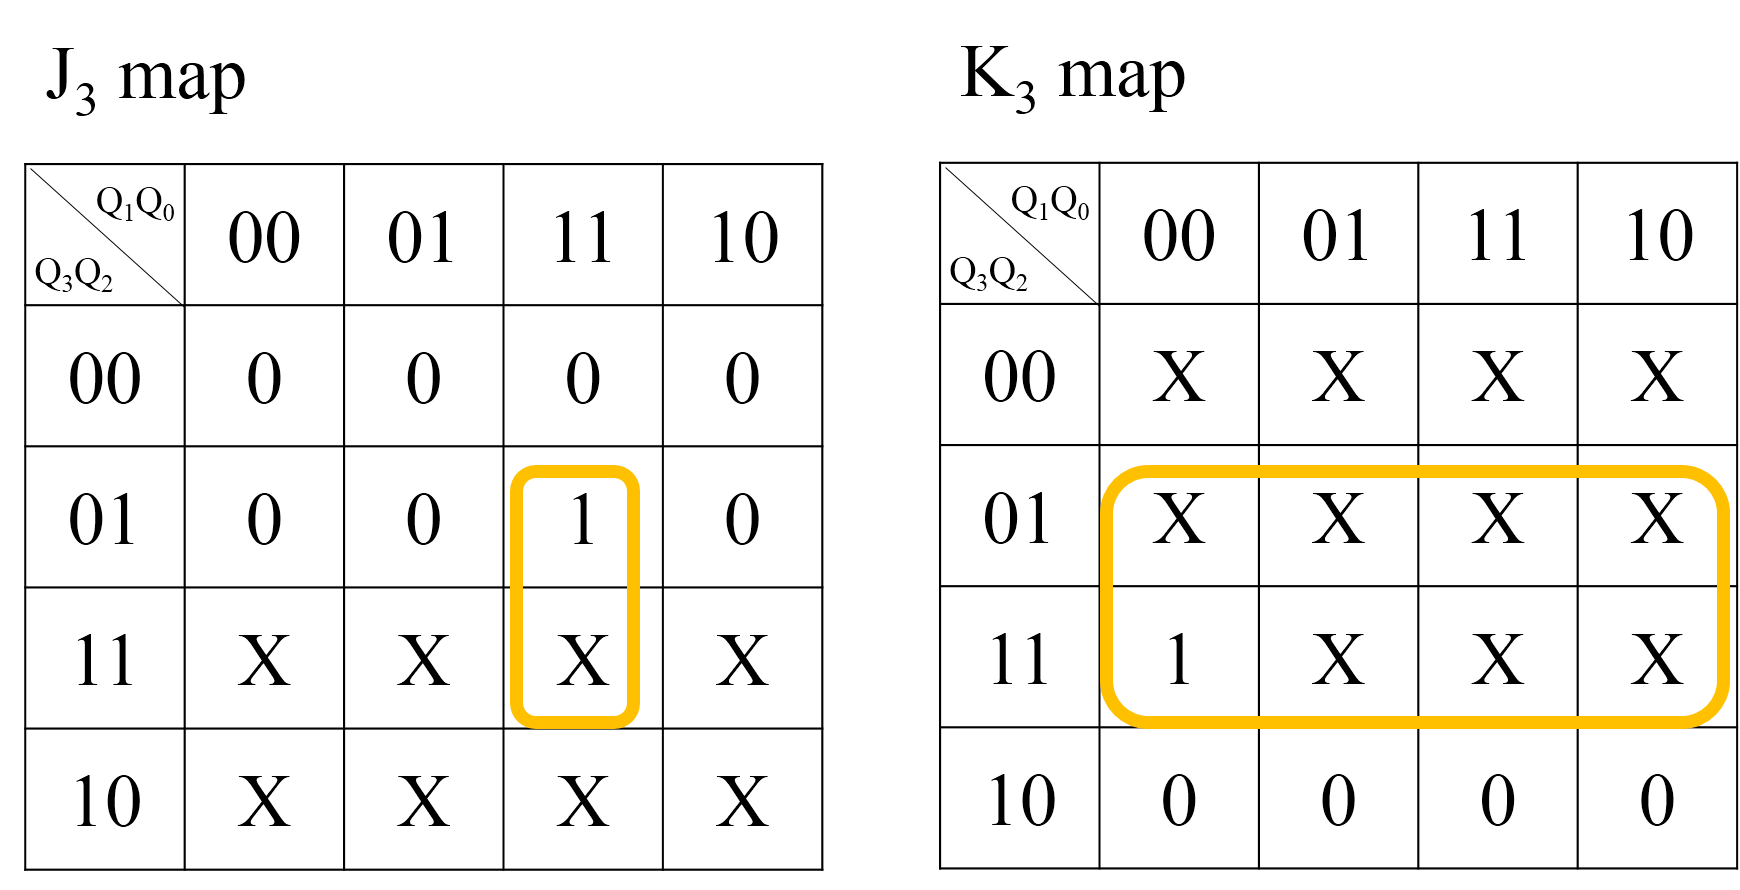
\includegraphics[scale=0.5]{4/k4.png}
\end{figure}

\newpage

\subsubsection{驱动方程}

$J_0 = 1$

$K_0 = 1$

$J_1 = Q_0$

$K_1 = Q_0$

$J_2 = Q_1 \cdot Q_0$

$K_2 = Q_1 \cdot Q_0 + Q_3 \cdot \overline{Q_1} \cdot \overline{Q_0}$

$J_3 = Q_2 \cdot Q_1 \cdot Q_0$

$K_3 = Q_2$

\subsubsection{电路图}

\begin{figure}[!hbp]
  \centering
  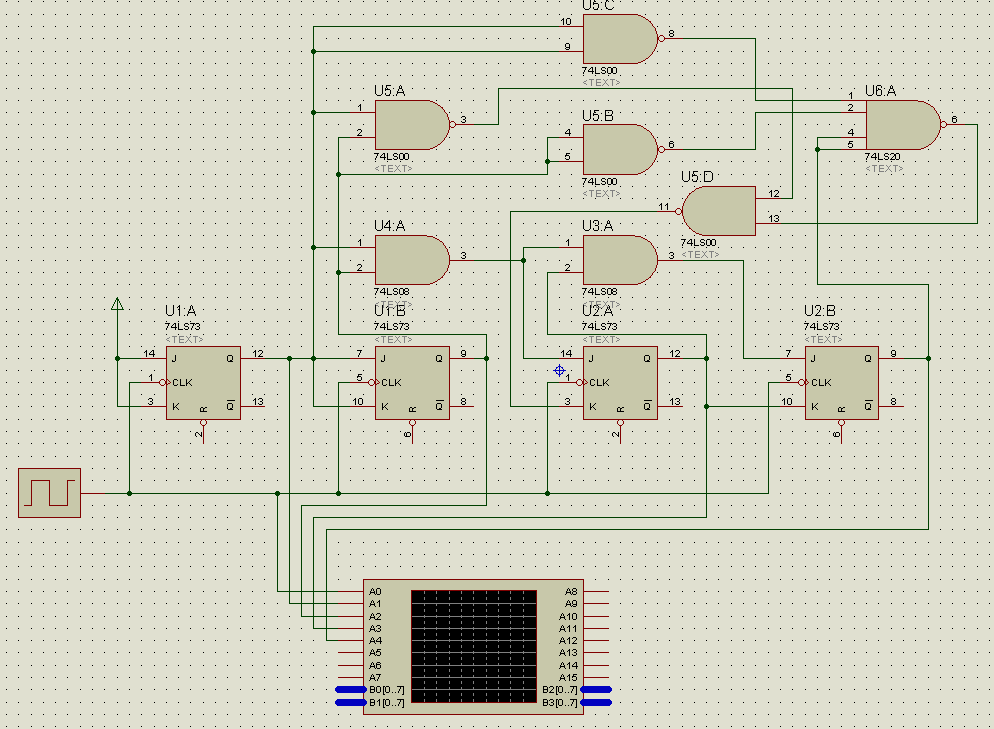
\includegraphics[scale=0.4]{4/1.png}
\end{figure}

\newpage

\subsubsection{Proteus 逻辑分析仪}

\begin{figure}[!hbp]
  \centering
  
\includegraphics[scale=0.5]{4/2.png}
\end{figure}

\subsubsection{实验板实现——逻辑分析仪}

\begin{figure}[!hbp]
  \centering
  \includegraphics[scale=0.5]{4/DS2_QuickPrint3.png}
\end{figure}

\end{document}
















